% Pipeline of the proposed study, laid out left to right for a slide.
% Content follows Figure 4.1 (dlsu-manuscript/chapter_4.tex, fig:pipeline) and Section 1.3 (Data preparation).
\documentclass[12pt,border=10pt]{standalone}
% Shared style for the slide figures: sans-serif text (Helvetica, close to the Arial of the charts),
% the same colors as charts.py, and the manuscript's table tools.
\usepackage[T1]{fontenc}
\usepackage[scaled]{helvet}
\renewcommand{\familydefault}{\sfdefault}
\usepackage{amsmath,amssymb}
\usepackage{sansmath}
\usepackage{xcolor}
\usepackage{booktabs,array}
\newcolumntype{L}[1]{>{\raggedright\arraybackslash}p{#1}}
\usepackage{tikz}
\usetikzlibrary{arrows.meta,positioning,calc}

\definecolor{ink}{HTML}{0B0B0B}
\definecolor{inktwo}{HTML}{52514E}
\definecolor{muted}{HTML}{898781}
\definecolor{gridc}{HTML}{E1E0D9}
\definecolor{basec}{HTML}{C3C2B7}
% one color per selection rule, in the fixed categorical order of the charts
\definecolor{cp}{HTML}{2A78D6}     % k-Changepoint (content)
\definecolor{sme}{HTML}{EB6834}    % SME (position)
\definecolor{posc}{HTML}{1BAF7A}    % positional (position)
\definecolor{rnd}{HTML}{EDA100}    % random (chance)
\definecolor{bocpd}{HTML}{E87BA4}  % k-BOCPD (content), categorical slot 5
\definecolor{temporal}{HTML}{6250D6}  % temporal information added to the mean (frame combinations figure)

\newcommand{\chip}[1]{\tikz[baseline=0.1ex]\fill[#1, rounded corners=1pt] (0,0) rectangle (0.32cm,0.32cm);}
\AtBeginDocument{\sansmath\color{ink}}
\hyphenpenalty=10000 \exhyphenpenalty=10000   % no hyphenated words on slides

\begin{document}
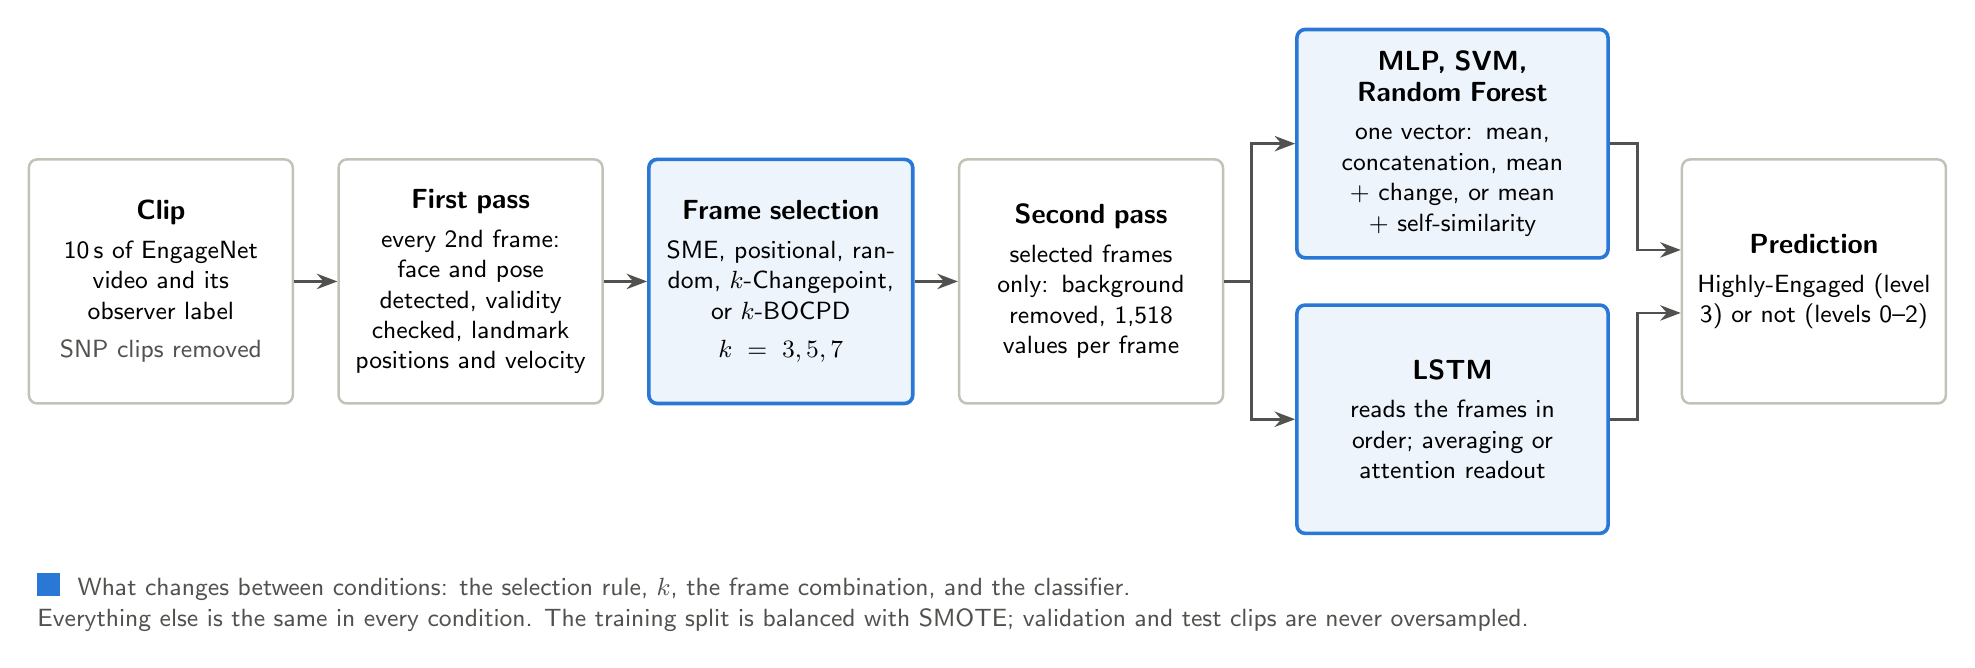
\begin{tikzpicture}[
   box/.style={draw=basec, line width=0.9pt, rounded corners=3pt, align=center, text width=3.0cm,
               minimum height=3.1cm, inner sep=5pt, font=\small, fill=white},
   var/.style={box, draw=cp, fill=cp!8, line width=1.3pt},
   arr/.style={-{Stealth[length=2.6mm]}, line width=1pt, color=inktwo}
]
   \node[box] (clip) {\textbf{\normalsize Clip}\\[3pt] 10\,s of EngageNet video and its observer label\\[3pt]\textcolor{inktwo}{SNP clips removed}};
   \node[box, right=0.55cm of clip] (scan) {\textbf{\normalsize First pass}\\[3pt] every 2nd frame: face and pose detected, validity checked, landmark positions and velocity};
   \node[var, right=0.55cm of scan] (select) {\textbf{\normalsize Frame selection}\\[3pt] SME, positional, random, $k$-Changepoint, or $k$-BOCPD\\[3pt] $k = 3, 5, 7$};
   \node[box, right=0.55cm of select] (second) {\textbf{\normalsize Second pass}\\[3pt] selected frames only: background removed, 1,518 values per frame};
   \node[var, text width=3.6cm, minimum height=2.9cm, anchor=west] (combo) at ($(second.east)+(0.9,1.75)$)
      {\textbf{\normalsize MLP, SVM, Random Forest}\\[3pt] one vector: mean, concatenation, mean + change, or mean + self-similarity};
   \node[var, text width=3.6cm, minimum height=2.9cm, anchor=west] (lstm) at ($(second.east)+(0.9,-1.75)$)
      {\textbf{\normalsize LSTM}\\[3pt] reads the frames in order; averaging or attention readout};
   \node[box, anchor=west, minimum height=3.1cm] (pred) at ($(combo.east |- second.east)+(0.9,0)$)
      {\textbf{\normalsize Prediction}\\[3pt] Highly-Engaged (level 3) or not (levels 0--2)};

   \draw[arr] (clip) -- (scan);
   \draw[arr] (scan) -- (select);
   \draw[arr] (select) -- (second);
   \draw[arr] (second.east) -- ++(0.35,0) |- (combo.west);
   \draw[arr] (second.east) -- ++(0.35,0) |- (lstm.west);
   \draw[arr] (combo.east) -- ++(0.35,0) |- ([yshift=0.4cm]pred.west);
   \draw[arr] (lstm.east) -- ++(0.35,0) |- ([yshift=-0.4cm]pred.west);

   \node[anchor=north west, font=\small, text=inktwo, align=left] at ($(clip.south west |- lstm.south)+(0,-0.35)$)
      {\textcolor{cp}{\rule{0.9em}{0.9em}}\ \ What changes between conditions: the selection rule, $k$, the frame combination, and the classifier.\\
       Everything else is the same in every condition. The training split is balanced with SMOTE; validation and test clips are never oversampled.};
\end{tikzpicture}
\end{document}
